
\section{Generative Adversarial Networks}

The goal of any generative model is to learn a probability distribution from data. Given a set of observed data $X$, we wish to recover the probability distribution $P_r$ that it was drawn from. If we were able to find $P_r$ exactly, that would mean we could draw unlimited samples from the same distribution that generated $X$. For example, if $X$ is a set of dog images, drawing new samples from its source distribution would be equivalent to generating entirely new images of dogs. 


In practice, we want to find $argmin_\theta(d(P_r, P_\theta))$, where $d$ is some measure of distance (divergence) between probability distributions. If we were to find $P_\theta=P_r$, then drawing a sample from $P_\theta$ would be equivalent to drawing a sample from $P$. In practice, we hope to find a sufficiently close $P_\theta$ so that drawing a sample from $P_\theta$ \textit{appears} equivalent to drawing a sample from $P_r$.

There are many approaches to generative modeling, such as PixelRNN~\cite{Oord2016}, PixelCNN~\cite{Oord2016a}, and Variational Autoencoders (VAE)~\cite{Pu2016}. In this paper however, we will focus on the Generative Adversarial Network~\cite{Goodfellow2017} and one of its most successful successors, the Wasserstein Generative Adversarial Network~\cite{Arjovsky2017}.

\subsection{Orginal GAN}

The GAN approach to generative modeling is unlike traditional approaches (PixelRNN, PixelCNN, VAE, etc.) in that its goal is not to find $P_\theta$. Rather, the goal is to find a function $G$ such that $G(z) \sim P_\theta, z \sim P_z~$ where $P_z$ is a \textit{previously known} probability distribution. In other words, GANs try to find a function that \textit{transforms} samples from a known distribution $P_z$ into samples from the target distribution $P_\theta$. We never actually find $P_\theta$, but that doesn't really matter since we are still able to draw samples from it. 

In the GAN architecture, two neural networks (a generator, $G$ and a discriminator, $D$) compete against each other (Figure \ref{fig:gan}). A common analogy for their relationship is that of a banker and a counterfeiter. The banker's goal is to discriminate between real and fake money while the counterfeiter's goal is to trick the banker into classifying his fake money as real. By participating in this game, the banker gets better at identifying fake money, and the counterfeiter gets better at manufacturing realistic fake money. In GANs, $G$ and $D$ play a similar game with each other until the samples generated by $G$ are so realistic enough that $D$ is forced to guess (with a 50\% chance of being correct) whether or not the sample is authentic. This can be formalized as a min-max game:

\begin{align}
	\label{eq:minmax}
	\underset{G}{min}~\underset{D}{max} L(D, G) =& \mathbb{E}_{x \sim P_r}~log(D(x)) + \mathbb{E}_{z \sim P_z}~log(1-D(G(z))) \nonumber \\
	=& \mathbb{E}_{x \sim P_r}~log~D(x) + \mathbb{E}_{x \sim P_\theta}~log~D(1-x) \nonumber \\ 
	=& \int_{x}^{} \frac{p_r(x)}{P_r + P_\theta(x)} + \int_{x}^{} \frac{P_\theta(x)}{P_r + P_\theta(x)} 
\end{align}

\begin{figure}[h!]
	\centering
	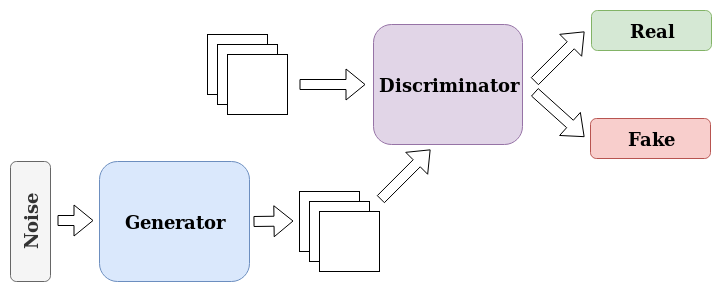
\includegraphics[width=0.8\linewidth]{media/gan.png}
	\caption{GAN Architecture. The Discriminator receives samples from the dataset and the generator and must accurately label them as real or fake.}
	\label{fig:gan}
\end{figure}

In other words, $D$ tries to \textit{maximize} the expected value for $log(D(x))$ over $x \sim P_r$ and $log(1-D(x))$ over $x \sim P_\theta$. At the same time, $G$ tries to \textit{minimize} the expected value of $log(1-D(x))$ over $x \sim P_\theta$. The solution to the game is a Nash Equilibrium and occurs when $D(x)=\frac{1}{2}$. We can derive this by finding the solution to $\frac{d f}{d D(x)} = 0$ where $f(D(x)) = P_r(x) log(D(x)) + P_\theta log(1-D(x)) = 0$, and considering the solution $P_r = P_\theta$: 

\begin{equation}
	\label{eq:optD}
	\begin{aligned}[c]
		\frac{d L}{d D(x)} =& \frac{1}{ln10} \left( \frac{P_r(x)}{D(x)} + \frac{(-1)P_\theta}{1-D(x)} \right) \\
		0 =& \frac{1}{ln10} \left( \frac{P_r(x)}{D(x)} - \frac{P_\theta}{1-D(x)} \right) \\
	\end{aligned}
	\qquad\Longleftrightarrow\qquad
	\begin{aligned}[c]
		P_\theta D(x) =& P_r(x) (1-D(x)) \\
		P_\theta D(x) =& P_r(x)-P_r(x) D(x) \\
		D(x)(P_\theta + P_r(x)) =& P_r(x) \\
		D(x) =& \frac{P_r(x)}{P_\theta + P_r(x)} 
	\end{aligned}
\end{equation}

Clearly, $P_r = P_\theta \Rightarrow D(x) = \frac{1}{2}$. Intuitively, this implies that the Generator's samples are so realistic that the Discriminator is forced to guess (with a 50\% chance of being correct) about their authenticity. 

Notice that minimizing the loss function is the same as minimizing the Jenson-Shannon Divergence, $d_j$, between $P_r$ and $P_\theta$:

\begin{align}
	d_j(P_r \Vert P_\theta) =& \frac{1}{2} \left( 2log2 + \int_{x}^{} \frac{p_r(x)}{P_r + P_\theta(x)} + \int_{x}^{} \frac{p_\theta(x)}{P_r + P_\theta(x)} \right) \nonumber \\
	=& log2 + \frac{1}{2} L(G, D) \nonumber \\
	L(G, D) =& 2d_j(P_r \Vert P_\theta) - 2log2
\end{align}

where $D(x) = \frac{1}{2}, x \sim P_\theta$. 

As an implementation detail, on the generator side, minimizing $-log~D(G(z))$ (or maximizing $log~D(G(z))$) is better than minimizing $log~D(1-G(z))$ since it's gradients are better for initial samples generated by $G$. So for the discriminator, we want to maximize $\mathbb{E}_{x \sim P_r}~log~D(x) + \mathbb{E}_{z \sim P_z} log D(1-G(z))$ and for the generator, we want to maximize $\mathbb{E}_{z \sim P_z}~log~D(1-G(z))$.

Since we are training two networks ($G$ and $D$) simultaneously, finding an equilibrium that optimizes both functions is difficult. Although images appear to be high-dimensional, studies show they are actually low-dimensional. Intuitively, we can think about how objects in an image are extremely dependent each other. For example, a picture of a person always contains two eyes relatively the same distance apart. The Jenson-Shannon Divergence do not support low-dimensional manifolds well. 
